\section{Hybrid ML + DL Model}
\label{sec:hybrid}

\subsection{Motivation}
The Phase 1 tree models and the Phase 2 sequence models summarise an engine's history in different ways. The Random Forest~\cite{breiman_2001_random} uses 57 engineered features over the last 10 cycles; the recurrent networks~\cite{hochreiter_1997_lstm,cho_2014_gru} read a raw 30-cycle window, as in earlier LSTM-based prognostics work~\cite{zheng_2017_lstm}. Phase 1 left three weaknesses: all models underpredicted engines with true RUL above 200 cycles, the rolling features saw only recent behaviour, and a few large errors dominated the RMSE. We tested whether stacking~\cite{wolpert_1992_stacked} the sequence models' estimates into a tree improves on both parts, and whether it is better than a plain average.

\subsection{Formal definition}
Let $x_{t-29:t}\in\mathbb{R}^{30\times14}$ be the scaled window of the 14 sensors ending at cycle $t$ of one engine, and $\phi(x)_t\in\mathbb{R}^{57}$ the Phase 1 rolling features (cycle, sensors, and the 10-cycle mean, standard deviation and slope of each sensor), computed from cycles $\le t$ only. A deep model $f_\theta$ gives the RUL estimate
\begin{equation}
d_t=f_\theta(x_{t-29:t}),
\end{equation}
and a tree regressor $g$ with the Phase 1 hyperparameters predicts
\begin{equation}
\hat y_t=g\big([\phi(x)_t,\ d_t,\ d^{\mathrm{gru}}_t]\big),
\end{equation}
where $d_t$ comes from an LSTM and $d^{\mathrm{gru}}_t$ from a GRU, each with the architecture selected in Section~\ref{sec:recurrent}. We used a scalar estimate rather than the hidden embedding because embeddings of separately trained networks live in different coordinate systems and cannot share one tree column, whereas $d_t$ is in cycles for every network. Two comparison hybrids were built: the average $\hat y_t=\tfrac12(d^{\mathrm{LSTM}}_t+\hat y^{\mathrm{RF}}_t)$ with no fitted weights (Hybrid~B), and a residual model in which $g$ predicts $y_t-d_t$ and $\hat y_t=d_t+g(\cdot)$ (Hybrid~C).

\subsection{Out-of-fold stacking}
If $f_\theta$ were trained on the same engines as $g$, its training predictions would be more accurate than its predictions for unseen engines, and $g$ would learn to trust $d_t$ too much. On our data, the selected LSTM had an MAE of 21.12 cycles on its own 80 training engines but 26.11 when each engine was predicted by a model that had not seen it. We therefore produced the training values of $d_t$ out-of-fold. The 80 training engines were split into $K=5$ folds by engine, with a seeded permutation. For fold $k$, a fresh network was trained on 56 of the other 64 engines and early-stopped on the remaining 8, with the scaler fitted on the 56. It then predicted the 16 engines of fold $k$. Neither the held-out fold nor the 20 validation engines was used to train or stop any fold model, and unit tests check this. For validation and test windows, $d_t$ is the mean of the 5 fold models, which never saw those engines and are of the same kind as the models behind the training values. All tables are joined on (engine, cycle) with assertions, never by position. The target was the true, uncapped RUL.

\subsection{Selection and evaluation}
Six variants were defined before any experiment (Table~\ref{tab:hybrid}). Selection used the lowest MAE over all windows of the 20 validation engines, with ties within 0.05 cycles going to the simpler variant. The 100 fixed validation points were reported after selection and not used to choose. The whole procedure (folds, 30 fold networks, trees) was repeated with seeds 42, 43 and 44. B-fold averages the same fold-mean $d_t$ as the stacked variants, so comparing it with B separates the effect of averaging from that of using the saved LSTM, whose early stopping used the validation engines.

\begin{figure}[t]
\centering
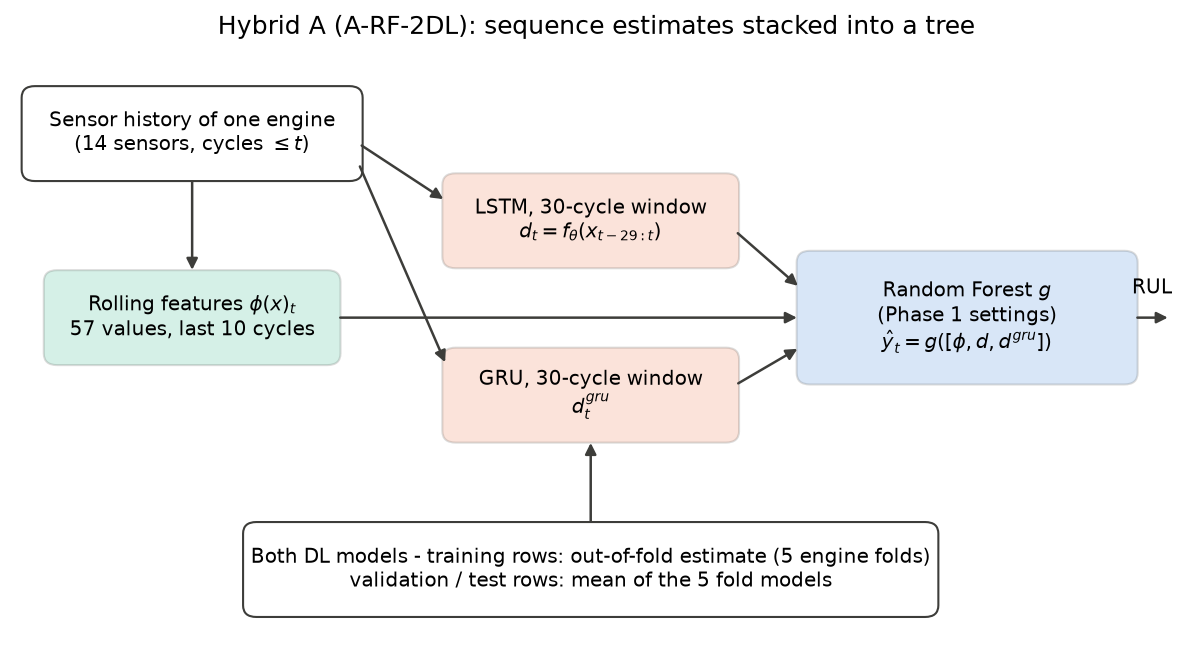
\includegraphics[width=\columnwidth]{../results/phase2/figures/hybrid_architecture.png}
\caption{Selected hybrid (A-RF-2DL). The LSTM and GRU estimates are stacked with the Phase 1 rolling features into a Random Forest. Training rows receive out-of-fold estimates; validation and test rows receive the mean of the five fold models.}
\label{fig:hybrid_arch}
\end{figure}

\begin{table}[t]
\centering
\caption{Validation results (cycles). Window MAE: all windows of the 20 validation engines (selection score), mean $\pm$ standard deviation over seeds 42--44. Points: the 100 fixed points, seed 42.}
\label{tab:hybrid}
\footnotesize
\resizebox{\columnwidth}{!}{%
\begin{tabular}{lccc}
\toprule
Model & Window MAE & Points MAE & Points RMSE\\
\midrule
\textbf{A-RF-2DL} (\texttt{hybrid\_v1}) & \textbf{25.28 $\pm$ 0.12} & 21.48 & 34.38\\
B, average (\texttt{hybrid\_avg\_v1}) & 25.68 $\pm$ 0.02 & 21.50 & 35.83\\
C-RF, residual (\texttt{hybrid\_resid\_v1}) & 25.89 $\pm$ 0.30 & 22.60 & 35.59\\
A-GB & 26.33 $\pm$ 0.13 & 23.07 & 35.90\\
A-RF & 26.38 $\pm$ 0.29 & 23.08 & 35.40\\
B-fold & 26.92 $\pm$ 0.23 & 23.03 & 37.00\\
\midrule
\texttt{lstm\_v1} & 26.38 & 19.41 & 34.45\\
LSTM, fold mean & 28.11 $\pm$ 0.52 & 21.75 & 36.22\\
Random Forest (Phase 1) & 27.77 $\pm$ 0.06 & 25.03 & 40.17\\
\bottomrule
\end{tabular}}
\end{table}

\begin{table}[t]
\centering
\caption{Component ablation: the same Random Forest on each feature group (seed 42, LSTM estimate only).}
\label{tab:hybrid_components}
\footnotesize
\resizebox{\columnwidth}{!}{%
\begin{tabular}{lcccc}
\toprule
Features & Count & Window MAE & Points MAE & Points RMSE\\
\midrule
DL estimate only & 1 & 28.72 & 24.93 & 38.10\\
Rolling only & 57 & 27.71 & 25.03 & 40.17\\
Both & 58 & 26.12 & 23.08 & 35.40\\
\bottomrule
\end{tabular}}
\end{table}

\subsection{Results}
The selection rule chose A-RF-2DL (Table~\ref{tab:hybrid}). Its window MAE of $25.28\pm0.12$ was lower than that of the Phase 1 Random Forest ($27.77\pm0.06$), its own fold-mean LSTM input ($28.11\pm0.52$) and the saved LSTM (26.38). Each gap is several times the seed standard deviation. On the 100 fixed points it reached an MAE of 21.48 ($21.72\pm0.31$ over seeds), 3.55 cycles below the Random Forest, and the lowest RMSE of all models (34.38). It did not beat the saved LSTM on these points (19.41), so we do not claim an improvement over the best deep model outside the selection set. The component ablation (Table~\ref{tab:hybrid_components}) shows that the two feature groups are complementary: the tree on both was better than on either alone. The tree's two most important features were $d^{\mathrm{gru}}_t$ (0.282) and $d_t$ (0.207), so it refined the sequence estimates rather than replacing them.

The simple average B came close: 0.40 cycles behind on the windows and equal on the points (21.50). With the same deep input, however, averaging (B-fold, $26.92\pm0.23$) was clearly worse than stacking, and the single-estimate stacked variants (A-RF, A-GB) did not beat B. The gain of the selected hybrid over B therefore depends on the second sequence estimate and is small.

The hybrid's early MAE (true RUL $>125$) was 41.52 cycles, against 49.33 for the Random Forest and 43.73 for the saved LSTM. Its late MAE was 15.83, against 12.55 for the LSTM. In the 200+ band (5 points) its mean signed error was $-116.3$ cycles, against $-123.3$ (Random Forest) and $-124.7$ (LSTM). The Phase 1 underprediction of high-RUL engines is therefore reduced only marginally, not solved.

As a negative control, a tree trained on in-sample $d_t$ weighted it more heavily (importance 0.388 against 0.309) and fitted the training engines more closely (MAE 12.53 against 13.80). With the saved LSTM's validation estimates, however, it was not worse on validation (window MAE 24.58 against 25.37). Early stopping limited the LSTM's in-sample optimism, so the control did not show a validation penalty on this split. We kept the out-of-fold procedure because only it gives the tree training inputs with the same error level as at inference. The main limitations are the 20 validation engines, the 5 points above 200 cycles, and the small mismatch between single out-of-fold estimates and the fold-mean estimates used at inference.
